%!TEX root = ../thesis.tex

\section{Algorithm explaination}\label{section:algorithm}

The polynomial-time algorithm introduced in \cite{PPPptime2016} describes a recursive procedure for reducing a red-black graph to an empty graph, if it admits a persistent phylogeny.
The recursion stops either when the base case is reached - empty graph (line \ref{algorithm:reduce:ifempty}) - or when the algorithm can't compute a successful c-reduction for \grb{} - the graph reaches a state of irreducibility (line \ref{algorithm:reduce:ifnosource}).

The procedure for a Reduce function is given below.

\begin{algorithm}[h]
  \caption{Reduce. Recursive reduction of a red-black graph.}\label{algorithm:reduce}

  \SetKwData{Source}{\ensuremath{s}}
  \SetKwData{Sc}{\ensuremath{S_{c}}}
  \SetKwInOut{Input}{Input}
  \SetKwInOut{Output}{Output}

  \Input{Red-black graph \grb{}}
  \Output{c-reduction of the graph \grb{}, if it exists}

  \BlankLine

  Remove singletons from \grb{}\;\label{algorithm:reduce:rmsingle}

  \BlankLine

  \If{\grb{} is empty}{\label{algorithm:reduce:ifempty}
    \Return $\langle$ $\rangle$\;
  }

  \BlankLine

  \If{\grb{} has a free character \character{}}{\label{algorithm:reduce:iffree}
    \grb{} $\gets$ Realize(\character[][-], \grb{})\;

    \Return $\langle$ \character[][-], Reduce(\grb{}) $\rangle$\;
  }

  \BlankLine

  \If{\grb{} has a universal character \character{}}{\label{algorithm:reduce:ifuniversal}
    \grb{} $\gets$ Realize(\character[][+], \grb{})\;

    \Return $\langle$ \character[][+], Reduce(\grb{}) $\rangle$\;
  }

  \BlankLine

  \If{\grb{} has k > 1 connected components}{\label{algorithm:reduce:ifdisconnected}
    \Return $\langle$ Reduce($\grb{}_{0}$), \dots, Reduce($\grb{}_{k-1}$) $\rangle$\;
  }

  \BlankLine

  \gm{} $\gets$ maximal reducible graph of \grb{}\;

  \hasse{} $\gets$ Hasse diagram for \gm{}\;

  \Source $\gets$ Find-initial-state(\hasse{})\;

  \BlankLine

  \If{\hasse{} has no safe source}{\label{algorithm:reduce:ifnosource}
    Abort\;
  }

  \BlankLine

  \Sc $\gets$ sequence of positive characters of \Source that are inactive in \grb{}\;

  \grb{} $\gets$ Realize(\Sc, \grb{})\;

  \BlankLine

  \Return $\langle$ \Sc, Reduce(\grb{}) $\rangle$\;
\end{algorithm}

The Reduce procedure computes signed character realizations with the support of a Realize function, which follows the definition of Realization (\ref{definition:realization}) and extends it to support a list of signed characters as input.

We will address the Find-initial-state procedure in detail in section \ref{section:safe-chains-sources}.

\subsection{Preparing the graph}\label{section:preparing-the-graph}

An explaination of lines \ref{algorithm:reduce:rmsingle} to \ref{algorithm:reduce:ifdisconnected} has already been provided in section \ref{section:grb}.

The first steps of the Reduce procedure (algorithm \ref{algorithm:reduce}) serve the purpose of bringing the red-black graph to a state which can't be "pruned" further.
Removing isolated vertices (singletons), realizing free and universal characters, and reducing each connected component of \grb{} separately is all part of preparing the graph for a more thorough analysis.

\subsection{Maximal reducible graph and Hasse diagram}\label{section:gm-hassediagram}

Let us introduce the concept of \emph{maximal} character. A character \character{} is maximal in a red-black graph \grb{} if $S(\character{}) \not\subset S(\character[i])$ for each inactive character \character[i] of \grb{}. Two maximal characters \character[0] and \character[1] can overlap, i.e., share common species, but clearly they can't be included in one another. Moreover, to clarify what we just described, we say that a character \character[0] includes another character \character[1] if $S(\character[0]) \supseteq S(\character[1])$.

The set of maximal characters of \grb{} is then used to build a maximal reducible graph \grbcm{} from it.

\begin{definition}[Maximal reducible graph]\label{definition:maximal-reducible-graph}
  Let \grb{} be a red-black graph and \cm{} its set of maximal characters.

  The maximal reducible graph \grbcm{}, \gm{} for short, is the red-black graph induced in \grb{} by the set \cm{} of characters.

  \gm{} consists of the subgraph of \grb{} that has the characters in \cm{} and the species of \grb{} adjacent to \cm{}.
\end{definition}

To be able to compute a successful c-reduction for a graph \grb{} we need to represent the set of species of its maximal reducible graph \gm{} as a Hasse diagram \cite{PPPptime2016}.
The Hasse diagram is used to represent partially ordered sets (poset), defined as $(P_{s}, \leq)$, where each element of $P_{s}$ is a vertex in the diagram and there exists an edge from a vertex $a$ to $b$ if and only if $a < b$ and there doesn't exist a vertex $c$ such that $a < c < b$.

The definition of Hasse diagram translates in our algorithm as a directed acyclic graph, where the vertices of $P_{s}$ are made up of the species of \gm{}.

\begin{definition}[Hasse diagram for \grbcm{}]\label{definition:hasse-diagram}
  Let \gm{} be a maximal reducible graph.

  The Hasse diagram \hasse{} for \gm{} is the Hasse diagram for the poset $(P_{s}, \leq)$ of the species of \gm{} ordered by the relation $\leq$.
  Two species \species[1] and \species[2] of $P_{s}$ are in a relation $\species[1] \leq \species[2]$ if $C(\species[1]) \subseteq C(\species[2])$
\end{definition}

Each vertex of a Hasse diagram \hasse{} consists of a set of species which share the same characters, while each edge \edge{v_{i}}{v_{i+1}} of the diagram is labeled by the set of positive characters that are in $v_{i+1}$ and not in $v_{i}$. When a character \character{} "is in" a vertex $v_{i}$, it means that all the species that label $v_{i}$ have the character \character{} in their set $C(\species{})$.

We show an example of maximal reducible graph and its corresponding Hasse diagram.

\begin{figure}[H]
  %!TEX root = ../thesis.tex

\centering
  \begin{subfigure}[b]{0.98\textwidth}
    \centering
      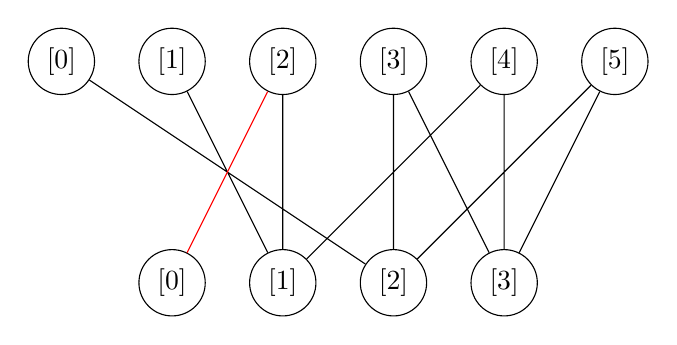
\begin{tikzpicture}
        {\tikzstyle{every node}=[circle, draw]
          \foreach \i in {0, ..., 5}
          {
            \node (s\i) at (\i*40pt, 80pt) {\species[\i]};
          }

          \foreach \j in {0, ..., 3}
          {
            \node (c\j) at (\j*40pt+40pt, 0) {\character[\j]};
          }
        }

        \draw
          (c3) -- (s3)
          (c3) -- (s4)
          (c3) -- (s5)
          (c1) -- (s1)
          (c1) -- (s2)
          (c1) -- (s4)
          (c2) -- (s0)
          (c2) -- (s3)
          (c2) -- (s5);

        \draw[red]
          (c0) -- (s2);
      \end{tikzpicture}

    \caption{Maximal reducible graph \gm{}}
    \label{figure:4:a}
  \end{subfigure}

  \bigskip

  \begin{subfigure}[b]{0.98\textwidth}
    \centering
      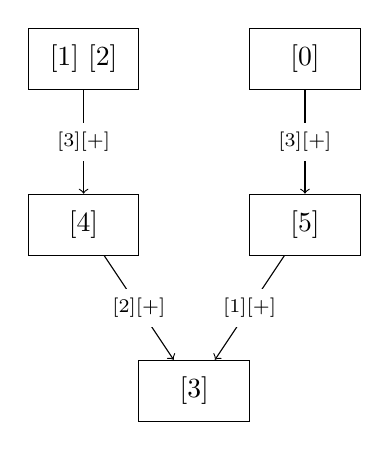
\begin{tikzpicture}
        {\tikzstyle{every node}=[rectangle, draw, minimum width=40pt, minimum height=22pt]
          \node (s1) at (0pt,  120pt) {\species[1] \species[2]};
          \node (s0) at (80pt, 120pt) {\species[0]};
          \node (s4) at (0pt,   60pt) {\species[4]};
          \node (s5) at (80pt,  60pt) {\species[5]};
          \node (s3) at (40pt,   0pt) {\species[3]};
        }

        {\tikzstyle{every node}=[fill=white, font=\scriptsize]
          \draw
            (s0) edge[->] node{\character[3][+]} (s5)
            (s1) edge[->] node{\character[3][+]} (s4)
            (s4) edge[->] node{\character[2][+]} (s3)
            (s5) edge[->] node{\character[1][+]} (s3);
        }
      \end{tikzpicture}

    \caption{Hasse diagram \hasse{} for \gm{}}
    \label{figure:4:b}
  \end{subfigure}


  \caption{Graph \gm{} and its Hasse diagram \hasse{}}\label{figure:4}
\end{figure}

\subsection{Safe chains and sources}\label{section:safe-chains-sources}

The algorithm operates on the Hasse diagram to find a \emph{safe source}, which is a necessary and sufficient condition for computing the \emph{initial state} of a tree $T_{A}$ solving the subgraph $\grbcm{} \cup A$.

Find-initial-state is the procedure for finding a safe source of a Hasse diagram.

A source in the diagram, i.e., a vertex of indegree 0, can be tested to be a safe source if and only if it's the source of a chain deemed to be safe. Moreover, we define a chain as a directed path from source to sink (vertex of outdegree 0).

To define the process to test if a chain is safe, we first need to introduce the concept of c-reduction of a chain. We say that the c-reduction of a chain $C = < v_{0}, \edge{v_{0}}{v_{1}}, v_{1}, \dots, \edge{v_{k-1}}{v_{k}}, v_{k} >$ of a diagram \hasse{} for \gm{}, alternating vertices and edges in the path, is the sequence of characters of $v_{0}$ ($C$'s source) and those labeling the edges \edge{v_{i}}{v_{i+1}} for $0 \leq i < k$.

\begin{definition}[Safe chain of a Hasse diagram]\label{definition:safe-chain}
  Let \hasse{} be the Hasse diagram for a graph \gm{}.
  Let $C$ be a chain of \hasse{}.

  A chain $C$ is safe in \hasse{} if its c-reduction applied to the graph \gm{} is feasible and the resulting graph doesn't include red \sg{}s.
\end{definition}

Then, the source $s$ of a safe chain can be subjected to the test for safe source if and only if its realization (i.e., the realization of the positive characters of $s$) on the graph \grb{} is feasible and the resulting graph doesn't include red \sg{}s.

Before listing the tests to be performed on a "realizable" source, let us premise that we worked, over the course of the project, on implementing a decent subset of the safe source tests.
The tests subset we implemented operates on graphs that have been reduced to maximal (\grbcm{}) right away; which means the first graph \grb{} will have only maximal characters.
The development of the remaining conditions to support minimal characters is currently in progress.

At last, we describe, in algorithmic form, the conditions for which a source can be considered safe.

\begin{algorithm}[hp]
  \caption{Find-initial-state. Select a safe source of a Hasse diagram, if it exists.}\label{algorithm:find-initial-state}

  \SetKw{Continue}{continue}
  \SetKwData{Source}{\ensuremath{source}}
  \SetKwData{SourceSpecies}{\ensuremath{s}}
  \SetKwInOut{Input}{Input}
  \SetKwInOut{Output}{Output}

  \Input{Hasse diagram \hasse{} for \grbcm{}}
  \Output{Safe source of \hasse{}, if it exists}

  \BlankLine

  \ForEach{safe chain of \hasse{}}{
    \Source $\gets$ the source of the chain\;
    \SourceSpecies $\gets$ a species in \Source\;

    \BlankLine

    \If{the realization of \SourceSpecies in \grb{} is not feasible or it induces red \sg{}s}{
      \Continue\;
    }

    \BlankLine

    \If{there exists a species $\SourceSpecies'$ in $\grbcm{} \cup A$ that consists of $C(\SourceSpecies)$ and is connected to only inactive characters}{\label{algorithm:find-initial-state:test1}
      \Return \Source\;
    }

    \BlankLine

    Add \Source to the list of feasible sources\;
  }

  \BlankLine

  \ForEach{\Source $\in$ list of feasible sources}{
    \SourceSpecies $\gets$ a species in \Source\;

    \BlankLine

    \If{there exists a species $\SourceSpecies'$ in $\grbcm{} \cup A$ that consists of $C(\SourceSpecies)$ + other maximal characters and is connected to only inactive characters}{\label{algorithm:find-initial-state:test2}
      \Return \Source\;
    }
  }

  \BlankLine

  \ForEach{\Source $\in$ list of feasible sources}{
    \SourceSpecies $\gets$ a species in \Source\;

    \BlankLine

    \If{there doesn't exist a species $\SourceSpecies'$ in $\grbcm{} \cup A$ that consists of $C(\SourceSpecies)$ + other active characters}{\label{algorithm:find-initial-state:test3}
      Abort\;
    }
  }

  \BlankLine

  \Source $\gets$ source having a species $\SourceSpecies$ whose realization frees all of its adjacent active characters\;

  \BlankLine

  \Return \Source\;
\end{algorithm}

\pagebreak
